%\documentclass{slides}
\documentclass{beamer}
\usepackage[utf8]{inputenc}
%\usepackage{portland}
\usepackage{graphicx}
%\usepackage{pdflscape}

%========Hierboven niets veranderen!========%

\usepackage[export]{adjustbox}% for the second solution
\usepackage{amsmath}
\usepackage{amsfonts}
\usepackage{amssymb}
\usepackage{mathtools}
\usepackage{scalerel}
\usepackage{tikz}
\usepackage[normalem]{ulem}
\usepackage{wisjab}

\setlength\fboxsep{4mm}
\setlength\fboxrule{0.8mm}

\definecolor{mygreen}{rgb}{0, 0.5, 0}
\def\gemph#1{{\color{mygreen}#1}}
\def\ck{\cellcolor{green!05}}

\def\lbt{} %Titel die linksboven verschijnt
\parindent=0pt
%\makesavenoteenv{tabular}
\renewcommand{\thefootnote}{\arabic{footnote}}

\DeclareMathOperator{\tr}{tr}
\DeclareMathOperator{\sgn}{sgn}
\DeclareMathOperator{\poly}{poly}
\DeclareMathOperator{\polylog}{polylog}
\DeclareMathOperator{\Rea}{Re}
\DeclareMathOperator{\Ima}{Im}
\renewcommand{\Re}{\Rea}
\renewcommand{\Im}{\Ima}

\def\vc#1{\boldsymbol{\mathsf{#1}}}
\def\mt#1{\kern0.025em\mathsf{#1}\kern0.025em}
\def\mtg#1{\kern0.6pt\slantbox[-0.25]{$#1$}\kern-0.6pt}

\def\1{\mathds1}
\def\d{\mathsf d}
\def\e{\mathsf e}
\def\i{\mathsf i}
\def\lambdai{{\lambda_{\sf i}}}
\def\lambdaf{{\lambda_{\sf f}}}

\def\A{\mt A}
\def\H{\mt H}
\def\HCD{\mt H_{\sf CD}}
\def\U{\mt U}

\def\+{\kern0.0833em}
\def\:{\kern-0.07em}
\def\>{\kern0.08em}
\def\<{\kern-0.08em}

\renewcommand{\thefootnote}{\arabic{footnote}}

\newenvironment{dia}[2]
{
	\begin{frame}
	\vspace{1mm}
	{\small #1}
	\hfill
    {\small\bf\textcolor{blue}{#2}}
	\vspace{3mm}
	\hrule
	\bigskip
}
{
	\vfill
	\end{frame}
}

\frenchspacing

\begin{document}

\setlength{\abovedisplayskip}{3mm}
\setlength{\belowdisplayskip}{3mm}
\setlength{\abovedisplayshortskip}{3mm}
\setlength{\belowdisplayshortskip}{3mm}

\begin{dia}{\lbt}{}
\vspace*{0.5cm}
\begin{center}
\begin{large}
AQC 10-06-2024 \\[1.25cm]
\end{large}
\begin{LARGE}
\textcolor{mygreen}{Gate-based counterdiabatic driving with complexity guarantees} \\[1.25cm]
\end{LARGE}
Dyon van Vreumingen (UvA / QuSoft, Amsterdam)
\end{center}
\end{dia}

\begin{dia}{\lbt}{Contents}
$ $\\
\begin{itemize}
    \setlength{\itemsep}{3mm}
    \item Counterdiabatic driving (CD) \pause
    \item Hardness of CD and need for fair comparison with adiabatic state preparation (ASP) \pause
    \item Gate-based CD algorithm and complexity bounds \pause
    \item Conclusion and outlook
\end{itemize}
\vspace{1.6cm}
\end{dia}

\begin{dia}{\lbt}{Counterdiabatic driving}
Say $\H(\lambda(t)) = \H_{\sf i} + f(\lambda(t)) \H_{\sf p}$ and we want eigenstate at $t = T$ \pause \\[4mm]
Infidelity caused by \gemph{nonadiabatic transitions} into other eigenstates \pause \\[4mm]
Idea: time-evolve with $\HCD(\lambda(t)) = \H(\lambda(t)) + \text{something}(t)$ such that transitions are \gemph{suppressed} and we can evolve faster \pause \\[4mm]
\begin{center}
    \begin{tabular}{ccc}
        adiabatic & non-adiabatic & counter-diabatic \\[2mm]
        
\includegraphics[scale=0.3]{fig/ober_a.pdf} &
        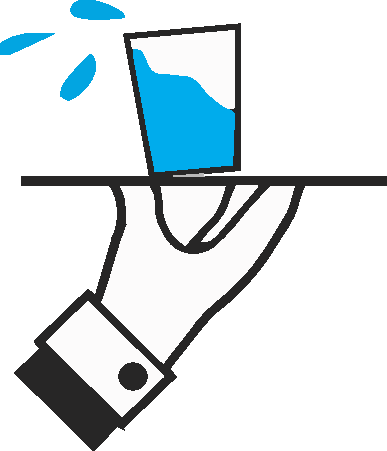
\includegraphics[scale=0.3]{fig/ober_b.pdf} &
        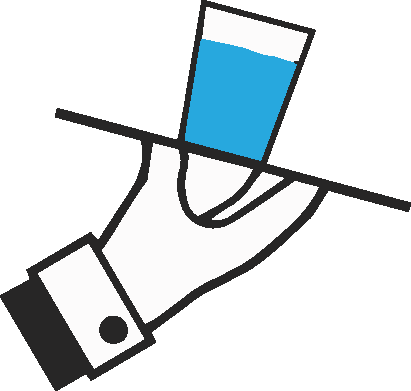
\includegraphics[scale=0.3]{fig/ober_c.pdf}
    \end{tabular}
\end{center}
\vspace{-1.4cm}
\end{dia}

\begin{dia}{\lbt}{Counterdiabatic driving}
Say $\H(\lambda(t)) = \H_{\sf i} + f(\lambda(t)) \H_{\sf p}$ and we want eigenstate at $t = T$ \\[4mm]
Infidelity caused by \gemph{nonadiabatic transitions} into other eigenstates \\[4mm]
Idea: time-evolve with $\HCD(\lambda(t)) = \H(\lambda(t)) + \gemph{\dot\lambda(t) \A(\lambda(t))}$ such that transitions are \gemph{suppressed} and we can evolve faster \\[4mm]
\begin{center}
    \begin{tabular}{ccc}
        adiabatic & non-adiabatic & counter-diabatic \\[2mm]
        
\includegraphics[scale=0.3]{fig/ober_a.pdf} &
        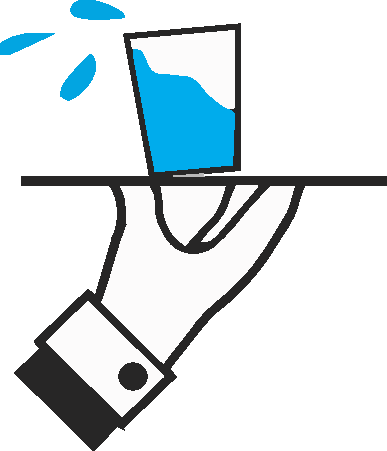
\includegraphics[scale=0.3]{fig/ober_b.pdf} &
        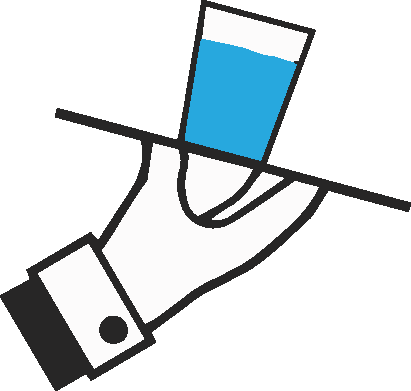
\includegraphics[scale=0.3]{fig/ober_c.pdf}
    \end{tabular}
\end{center}
\vspace{-1.4cm}
\end{dia}

\begin{dia}{\lbt}{Counterdiabatic driving}
$\A(\lambda)$ can be determined from requirement of transitionless driving for \gemph{any driving time $T$} (i.e. also in limit $T\to0$): \pause
\begin{align*}
    \sum_n \ket{n(\lambdaf)}\bra{n(\lambdai)} &\overset{{\color{white}T\to\>0}}{=} \mathcal T\exp \bigg[ \!-\!\i \int_0^{{\color{mygreen}T}} \d t \, [\mt H(\lambda(t)) + \dot\lambda(t) \mt A(\lambda(t))] \bigg] \nonumber \\[2mm]
    &\overset{{\color{mygreen}T}\to\>0}{=} \mathcal T\exp \bigg[ \!-\!\i \int_\lambdai^\lambdaf \d\lambda \, \mt A(\lambda) \bigg]
\end{align*}
$ $\\ \pause
Identify $\mt A(\lambda) = \i \> \partial_\lambda$ (generator of translations in $\lambda$ space) \pause \\[4mm]
$\A$ is known as \gemph{adiabatic gauge potential} (AGP)
\vspace{-6mm}
\end{dia}

\begin{dia}{\lbt}{Hardness of CD}
However, computing $\mt A$ is \gemph{hard}! \pause \\[4mm]
Typically, $\mt A$ is nonlocal and contains high-rank interactions \pause \\[4mm]
Methods to approximate AGP for imperfect but improved driving \pause
\begin{itemize}
    \item Variational methods \pause
    \item Lanczos algorithm / Krylov space methods \pause
\end{itemize}
$ $\\
Works well for simple systems... \pause \\[4mm]
...but for complex systems, compute time scales like $\sim\mathrm{dim}(\mathcal H)^2$
%\vspace{-1cm}
\end{dia}

\begin{dia}{\lbt}{Hardness of CD}
This begs the question: \pause
\begin{center}
    \gemph{is counterdiabatic driving really worthwhile?} \pause
\end{center}
By this we mean:
\begin{itemize}
    \item does the computational complexity needed to boost fidelity through CD scale favourably... \pause
    \item ...as compared to simply increasing the evolution time in ASP?
\end{itemize}
$ $\\ \pause
By the way, how do we compare complexities? \\[4mm] \pause
We count \gemph{quantum gates} on fault-tolerant QC
\vspace{-1cm}
\end{dia}

\begin{dia}{\lbt}{Complexity of ASP}
%Denote $\|\mt O\|_{\infty, p} = \big( \int_\lambdai^\lambdaf \d\lambda \, \|\mt O(\lambda)\|^p \big)^{1 / p}$. Then f
For ASP, we know the the JRS bound
\begin{align*}
    T \geq O(\Delta^{-3} \epsilon^{-1} 
    %\|\partial_\lambda \mt H\|_{\infty, 2}^2
    ) \Rightarrow |\braket{n(\lambdaf)}{\psi(T)}|^2 \geq 1 - \epsilon^2
\end{align*}
where $\Delta$ is the \gemph{minimum gap} around $\ket{n(\lambda)}$ along the path \\[2mm] \pause
To turn this into quantum gates, we trotterise
\begin{align*}
    \mathcal T\exp \bigg[ \!-\!\i \int_0^T \d t \, \mt H(\lambda(t)) \bigg] \approx \prod_j \exp[-\i \> \mt H_j \> \delta t_j]
\end{align*} \pause
With a $k$\textsuperscript{th}-order \gemph{Lie-Suzuki-Trotter formula}\pause, we need
\begin{align*}
    O\Big( \Delta^{-(3 + \frac3{2k})} \epsilon^{-(1 + \frac1k)} \, (25/3)^k \Big)
\end{align*}
quantum gates to obtain fidelity $\geq 1 - \epsilon^2$
\vspace{-1cm}
\end{dia}

\begin{dia}{\lbt}{}
\vspace{2.5cm}
\begin{center}
\begin{LARGE}
\textcolor{mygreen}{Gate-based counterdiabatic driving}
\end{LARGE}
\end{center}
\vspace*{1.5cm}
\end{dia}

\begin{dia}{\lbt}{Gate-based CD}
Goal: to approximate the unitary
\begin{align*}
    \mt U(\lambdaf, \lambdai) = \sum_n \ket{n(\lambdaf)}\bra{n(\lambdai)} = \mathcal T \exp \bigg[ \! -\!\i \int_\lambdai^\lambdaf \d\lambda \, \mt A(\lambda)) \bigg]
\end{align*}
with some unitary $\tilde{\mt U}(\lambdaf, \lambdai)$ that can be implemented on a fault-tolerant QC \\[6mm] \pause
We upper bound euclidean distance $\|(\mt U - \tilde{\mt U})\ket{n(\lambdai)}\|$, since
\begin{align*}
    \|(&\mt U - \tilde{\mt U})\ket{n(\lambdai)}\| \leq \epsilon \nonumber \\[2mm]
    &\Rightarrow |\bra{n(\lambdai)} \mt U\t \tilde{\mt U} \ket{n(\lambdai)}|^2 \geq 1 - \epsilon^2
\end{align*}
\vspace*{-1.4cm}
\end{dia}

\begin{dia}{\lbt}{Time-integral AGP}
\gemph{Time-integral form} of AGP
\begin{align*}
    \A = \frac12 \lim_{\eta\to0} \int_{-\infty}^\infty \d\tau \, \e^{-\eta|\tau|} \sgn(\tau) \, \e^{-\i\H\tau} \partial_\lambda \H \+ \e^{\i\H\tau} \\[-8mm]
\end{align*} \pause
$ $\\[-2mm]
has matrix elements (in energy eigenbasis)
\begin{align*}
    %\bra m \A \ket n &= \frac12 \lim_{\eta\to0} \int_{-\infty}^\infty \d\tau \, \e^{-\eta|\tau|} \sgn(\tau) \, \e^{-\i(E_m - E_n)\tau} \bra m \partial_\lambda \H \ket n \\[2mm]
    \bra m \mt A \ket n = \lim_{\eta\to0} \frac{\omega_{mn}}{\i(\omega_{mn}^2 + \eta^2)} \bra m \partial_\lambda \mt H \ket n \quad \quad \omega_{mn} = E_m - E_n
\end{align*} \pause
$ $\\[2mm]
At the same time, by the Hellman-Feynman theorem,
\begin{align*}
    \bra m \A \ket n = \i \bra m \partial_\lambda \ket n = \frac{\bra m \partial_\lambda\H \ket n}{\i \+ \omega_{mn}}
\end{align*} 
\vspace{-1.4cm}
\end{dia}

\begin{dia}{\lbt}{Algorithm}
We construct a gate-based algorithm in three steps \pause
\begin{enumerate}
    \item \gemph{Regularise} and \gemph{truncate} integral expression:
    \begin{align*}
        \A \approx \A_{\eta, a} = \frac12 \int_{-a}^a \d\tau \, \e^{-\eta|\tau|} \sgn(\tau) \, \e^{-\i\H\tau} \partial_\lambda \H \+ \e^{\i\H\tau}
    \end{align*}
    for $\eta, a \geq 0$ \pause
    \item Approximate the time integral with a \gemph{sum}:
    \begin{align*}
        \A_{\eta, a}(\lambda) \approx \A_{\eta, a}^{M, q}(\lambda) = \sum_{\kappa = -M}^M \sum_{\alpha = 0}^q \mt C_{\kappa, \alpha}(\lambda)
    \end{align*}
\end{enumerate}
\vspace{0.65cm}
\end{dia}

\begin{dia}{\lbt}{Algorithm}
We construct a gate-based algorithm in three steps
\begin{enumerate}
    \setcounter{enumi}{2}
    \item Approximate time-ordered exponential
    \begin{align*}
        \mt U_{\eta, a}^{M, q}(\lambdaf, \lambdai) = \mathcal T \exp\big[ \!-\!\i \int_\lambdai^\lambdaf \d\lambda \, \A_{\eta, a}^{M, q}(\lambda) \big]
    \end{align*}
    with a \gemph{Lie-Suzuki-Trotter} (LST) formula
    \begin{align*}
        \mt U_{\eta, a}^{M, q}(\lambdaf, \lambdai) \approx \tilde{\mt U}(\lambdaf, \lambdai) = \prod_j \exp[-\i \> \mt C_{\kappa_j, \alpha_j}(\lambda_j) \> \delta\lambda_j]
    \end{align*}
\end{enumerate} \pause
By a triangle equality, the total error is then at most
\begin{align*}
    \|(\mt U - \tilde{\mt U})\ket{n(\lambdai)}\| &\leq \|(\mt U - \mt U_{\eta, a})\ket{n(\lambdai)}\| \\
    &+ \|(\mt U_{\eta, a} - \mt U_{\eta, a}^{M, q})\ket{n(\lambdai)}\| + \|(\mt U_{\eta, a}^{M, q} - \tilde{\mt U})\ket{n(\lambdai)}\|
\end{align*}
\vspace{-1cm}
\end{dia}

\begin{dia}{\lbt}{1. Regularisation and truncation}
Regularisation
\begin{align*}
    \bra m \A_{\eta, \infty} \ket n = \frac{\omega_{mn}}{\i (\omega_{mn}^2 + \eta^2)} \bra m \partial_\lambda \mt H \ket n \quad \quad \omega_{mn} = E_m - E_n
\end{align*}
has effect of suppressing only those transitions with $|\omega_{mn}| \gg \eta$ \\[4mm] \pause
But we need to suppress only the transitions from the \gemph{$n$-th energy level}! \\[4mm] \pause
Truncation introduces an additional error $\sim \e^{-\eta a}$\pause; this leads to
\begin{align*}
    \eta &\leq O(\Delta^{3/2}\epsilon^{1/2}), \quad a \geq \tilde O(1 / \eta) \\[2mm]
    & \Rightarrow \|(\mt U - \mt U_{\eta, a})\ket{n(\lambdai)}\| \leq \epsilon
\end{align*}
\vspace{-1cm}
\end{dia}

\begin{dia}{\lbt}{2. Weighted sum approximation}
Riemann sum \pause
\begin{center}
    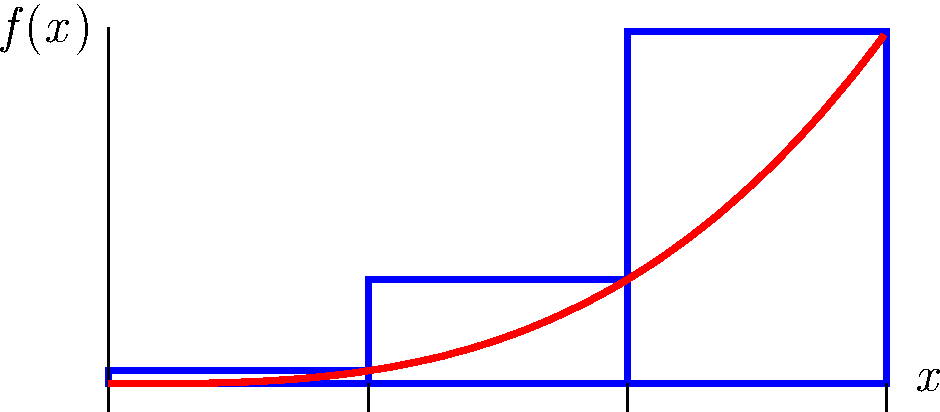
\includegraphics[width=0.7\textwidth]{fig/RightRiemann.pdf}
\end{center} \pause
\vspace{-2mm}
\begin{align*}
    \mt A_{\eta, a}^{M, 0} = \frac12 \sum_{\kappa = -M}^M \delta\tau_\kappa \> \e^{-\eta|\tau_\kappa|} \sgn\tau_\kappa \> \e^{-\i \mt H \tau_\kappa} \partial_\lambda \mt H \> \e^{\i \mt H \tau_\kappa}
\end{align*} \pause
\vspace{-2mm}
\begin{align*}
    M \geq O(\eta^{-2} \epsilon^{-1}) \Rightarrow \|(\mt U_{\eta, a} - \mt U_{\eta, a}^{M, 0})\ket{n(\lambdai)}\| \leq \epsilon
\end{align*}
\vspace{-1.4cm}
\end{dia}

\begin{dia}{\lbt}{2. Weighted sum approximation}
Trapezoidal rule \pause
\begin{center}
    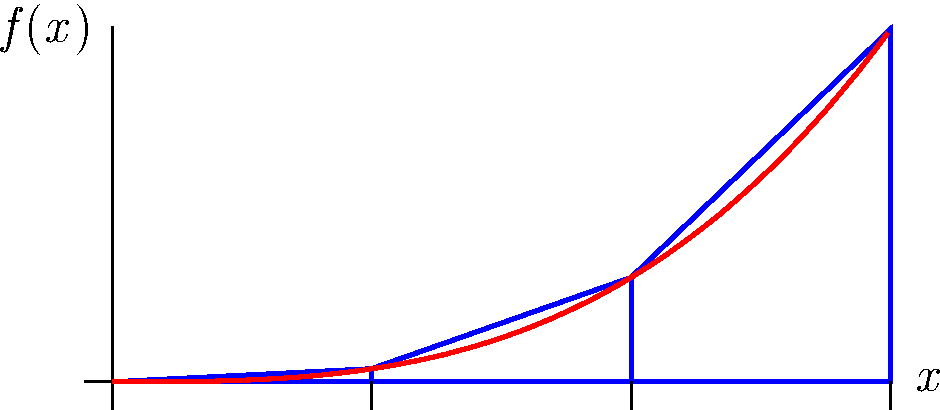
\includegraphics[width=0.7\textwidth]{fig/TrapRiemann.pdf}
\end{center} \pause
\vspace{-2mm}
\begin{align*}
    \mt A_{\eta, a}^{M, 1} = \frac12 \sum_{\kappa = -M}^M \frac{\delta\tau_\kappa}2 \> \big( \e^{-\eta|\tau_\kappa|} \sgn\tau_\kappa \> \e^{-\i \mt H \tau_\kappa} \partial_\lambda \mt H \> \e^{\i \mt H \tau_\kappa} + (\tau_\kappa \leftrightarrow \tau_{\kappa - 1}) \big)
\end{align*} \pause
\vspace{-2mm}
\begin{align*}
    M \geq O(\eta^{-3/2} \epsilon^{-1/2}) \Rightarrow \|(\mt U_{\eta, a} - \mt U_{\eta, a}^{M, 1})\ket{n(\lambdai)}\| \leq \epsilon
\end{align*}
\vspace{-1.4cm}
\end{dia}

\begin{dia}{\lbt}{2. Weighted sum approximation}
This pattern can be continued... \pause
\begin{align*}
    \mt A_{\eta, a}^{M, q} = \frac12 \sum_{\kappa = -M}^M \sum_{\alpha = 0}^q \, \delta\tau_\kappa w_{\kappa, \alpha} \big( \e^{-\eta|\tau_{\kappa, \alpha}|} \sgn\tau_{\kappa, \alpha} \> \e^{-\i \mt H \tau_{\kappa, \alpha}} \partial_\lambda \mt H \> \e^{\i \mt H \tau_{\kappa, \alpha}}) \big)
\end{align*} \pause
with $\sum_{\alpha = 0}^q w_{\kappa, \alpha} = 1$ \\[6mm] \pause
Weights $w_{\kappa, \alpha}$ only depend on our choice of $\tau_{\kappa, \alpha}$! \\[6mm] \pause
In the end, we get
\begin{align*}
    M \geq O\big( \eta^{-1 - \frac1{q + 1}} \epsilon^{-\frac1{q + 1}} (q + 1)^{-1} \big) \Rightarrow \|(\mt U_{\eta, a} - \mt U_{\eta, a}^{M, q})\ket{n(\lambdai)}\| \leq \epsilon
\end{align*}
\vspace{-0.8cm}
\end{dia}

\begin{dia}{\lbt}{2. Weighted sum approximation}
This pattern can be continued... 
\begin{align*}
    \mt A_{\eta, a}^{M, q} = \frac12 \sum_{\kappa = -M}^M \sum_{\alpha = 0}^q \, \underbrace{\delta\tau_\kappa w_{\kappa, \alpha} \big( \e^{-\eta|\tau_{\kappa, \alpha}|} \sgn\tau_{\kappa, \alpha} \> \e^{-\i \mt H \tau_{\kappa, \alpha}} \partial_\lambda \mt H \> \e^{\i \mt H \tau_{\kappa, \alpha}}) \big)}_{{} = \mt C_{\kappa, \alpha}}
\end{align*}
$ $\\[-4mm]
with $\sum_{\alpha = 0}^q w_{\kappa, \alpha} = 1$ \\[6mm]
Weights $w_{\kappa, \alpha}$ only depend on our choice of $\tau_{\kappa, \alpha}$! \\[6mm]
In the end, we get
\begin{align*}
    M \geq O\big( \eta^{-1 - \frac1{q + 1}} \epsilon^{-\frac1{q + 1}} (q + 1)^{-1} \big) \Rightarrow \|(\mt U_{\eta, a} - \mt U_{\eta, a}^{M, q})\ket{n(\lambdai)}\| \leq \epsilon
\end{align*}
\vspace{-0.9cm}
\end{dia}

\begin{dia}{\lbt}{3. Lie-Suzuki-Trotter expansion}
Trotter expansions serve to approximate
\begin{align*}
    \mathcal T \exp[-\i \int_\lambdai^\lambdaf \d\lambda \sum_{\kappa, \alpha} \mt C_{\kappa, \alpha}(\lambda)] 
    \approx \prod_j \exp[-\i \mt C_{\kappa_j, \alpha_j}(\lambda_j) \> \delta\lambda_j]
\end{align*} \pause
One can construct a $k$\textsuperscript{th}-order LST formula $\tilde{\mt U}_k$ with
\begin{align*}
    \tilde O\bigg( \frac{M \> q}{\eta^{1 + \frac1{2k}}\epsilon^{\frac1{2k}}} (25/3)^k \bigg)
\end{align*}
quantum gates to guarantee 
\begin{align*}
    \| \mathcal T \exp[-\i \int_\lambdai^\lambdaf \d\lambda \sum_{\kappa, \alpha} \mt C_{\kappa, \alpha}(\lambda)] - \tilde{\mt U}_k(\lambdaf, \lambdai) \| \leq \epsilon
\end{align*}
\vspace*{-1cm}
\end{dia}

\begin{dia}{\lbt}{Quantum gate complexity}
Putting everything together:
\begin{align*}
    M \> q &\leq O\big( \eta^{-1 - \frac1{q + 1}} \epsilon^{-\frac1{q + 1}} \big) \nonumber \\
    \eta &\leq O(\Delta^{3/2}\epsilon^{1/2})
\end{align*}
$ $\\[-8mm] \pause
\begin{align*}
    \Rightarrow \quad\quad &\tilde O\bigg( \frac{M \> q}{\eta^{1 + \frac1{2k}}\epsilon^{\frac1{2k}}} (25/3)^k \bigg) \nonumber \\[2mm]
    = {} &\tilde O\Big( \Delta^{-(3 + \frac3{4k} + \frac3{2(q + 1)})} \epsilon^{-(1 + \frac3{4k} + \frac3{2(q + 1)})} \, (25/3)^k \Big)
\end{align*}

to guarantee $|\bra{n(\lambdaf)} \tilde{\mt U} \ket{n(\lambdai)}|^2 \geq 1 - \epsilon^2$
\vspace{-0.2cm}
\end{dia}

\begin{dia}{\lbt}{}
\vspace{2.5cm}
\begin{center}
\begin{LARGE}
\textcolor{mygreen}{So what do we have?}
\end{LARGE}
\end{center}
\vspace*{1.5cm}
\end{dia}

\begin{dia}{\lbt}{Conclusion}
Gate-based ASP:
\begin{align*}
    O\Big( \Delta^{-(3 + \frac3{2k})} \epsilon^{-(1 + \frac1k)} \, (25/3)^k \Big)
\end{align*}
\pause Gate-based CD:
\begin{align*}
    \tilde O\Big( \Delta^{-(3 + \frac3{4k} + \frac3{2(q + 1)})} \epsilon^{-(1 + \frac3{4k} + \frac3{2(q + 1)})} \, (25/3)^k \Big)
\end{align*}
where $q$ can be made big cheaply \\[5mm] \pause
Scaling is almost the same for ASP and CD \\[5mm] \pause
``Shortcut to adiabaticity'' turns out not to be much of a shortcut after all...
\vspace{-0.6cm}
\end{dia}

\begin{dia}{\lbt}{Outlook}
Does this mean that CD is useless? \pause No \pause
\begin{itemize}
    \item There might be a better gate-based CD algorithm and/or better bounds \pause
    \item However, result suggests that there may not be much to gain with CD in a general, gate-based, worst-case setting \pause
    \item Since CD is really a coordinate change from time to $\lambda$ space, some kind of ``no free lunch'' phenomenon seems likely \pause
    \item Nonetheless, if quantum resources are scarce, CD with precomputed AGP can be useful \pause
    \item Eigenstate-specific AGP approximations seem promising (perhaps even crucial?)
\end{itemize}

\vspace{-1cm}
\end{dia}

\begin{dia}{\lbt}{}
\vspace{2.0cm}
\begin{center}
\begin{LARGE}
\textcolor{mygreen}{Thank you!}
\end{LARGE}
$ $\\[2.5cm]
Special thanks to Kareljan Schoutens, Takuya Hatomura and \\ Jan St\v{r}ele\v{c}ek
\end{center}
\vspace*{-0.5cm}
\end{dia}

\end{document}